\section{Low statistics and complementary results}
\label{app:add_plots}

In this appendix we collect some additional plots, in the same format of those
presented in figures~\ref{fig:atlaszhighmass49fb}--\ref{fig:cmsZ13TeV},
specifically: figure~\ref{fig:atlaszhighmass49fb-lowstat} is the same as
figure~\ref{fig:atlaszhighmass49fb}, but for a low-statistic MC run;
figure~\ref{fig:cmsdy2d11_bins12} is the same as
figure~\ref{fig:cmsdy2d11_bins3456}, but for the two missing lepton-pair
invariant mass bins,
$\SI{20}{\giga\electronvolt}<M_{\ell\bar\ell}<\SI{30}{\giga\electronvolt}$ and
$\SI{30}{\giga\electronvolt}<M_{\ell\bar\ell}<\SI{45}{\giga\electronvolt}$;
and figure~\ref{fig:atlastop-rap} is the same as figure~\ref{fig:atlastop},
but for the distributions in the rapidity of the top quark, $y_{\mathrm{t}}$,
and in the rapidity of the top-quark pair, $y_{\mathrm{t}\bar{\mathrm{t}}}$. In this
case the factorisation and renormalisation scales are kept equal to
$H_\mathrm{T}/4$, see section~\ref{sec:toppair}.

%-------------------------------------------------------------------------------
\begin{figure}[!t]
    \centering
    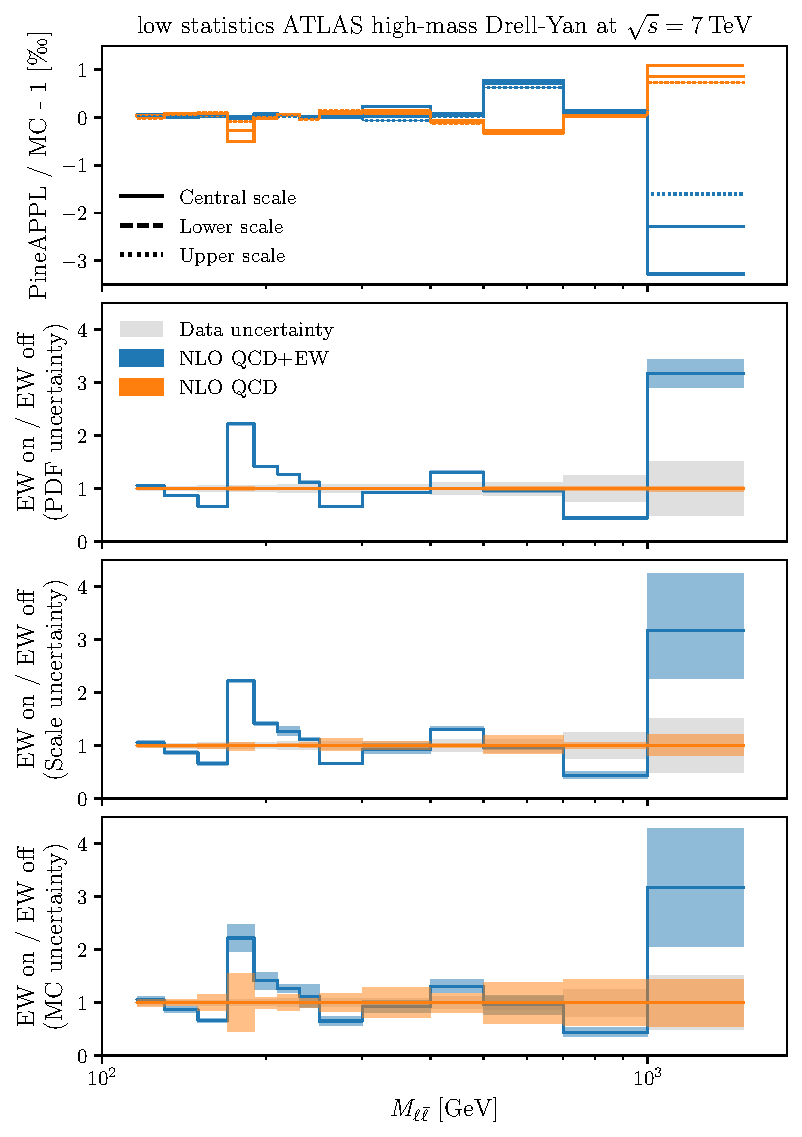
\includegraphics[width=0.46\textwidth]{figures/pineappl_ATLASZHIGHMASS49FB_lowstat}\\
    \caption{Same as figure~\ref{fig:atlaszhighmass49fb}, but for a
    low-statistics MC run.}
    \label{fig:atlaszhighmass49fb-lowstat}
\end{figure}
%-------------------------------------------------------------------------------

%-------------------------------------------------------------------------------
\begin{figure}[!p]
    \centering
    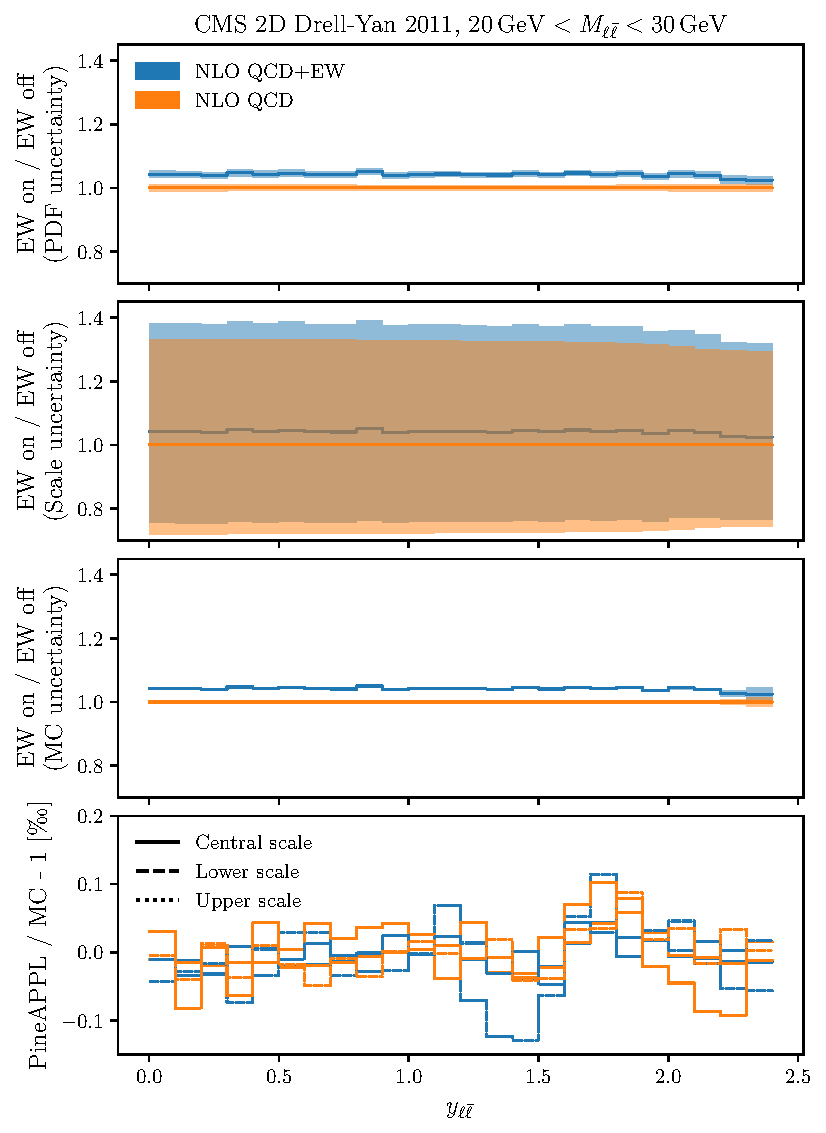
\includegraphics[width=0.46\textwidth]{figures/pineappl_CMSDY2D11_bin1}%
    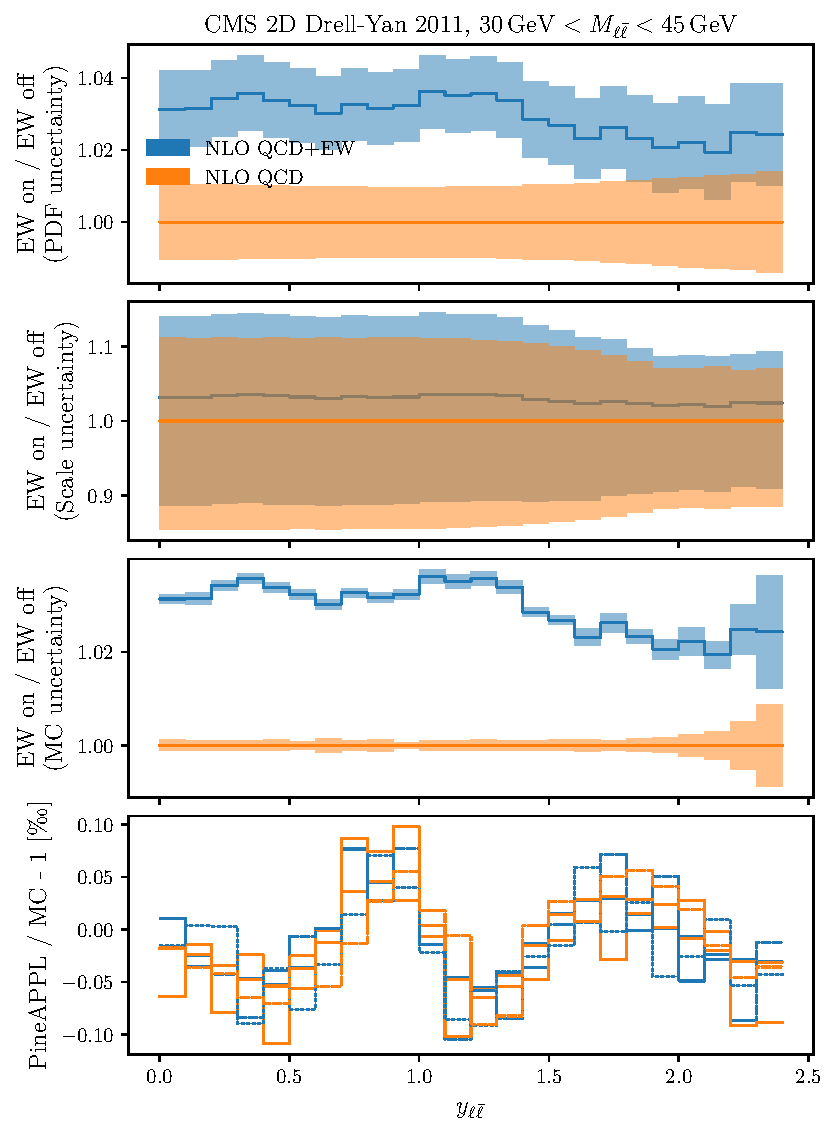
\includegraphics[width=0.46\textwidth]{figures/pineappl_CMSDY2D11_bin2}\\
    \caption{Same as figure~\ref{fig:cmsdy2d11_bins3456}, but for the two missing
      lepton-pair invariant mass bins,
      $\SI{20}{\giga\electronvolt}<M_{\ell\bar\ell}<\SI{30}{\giga\electronvolt}$ and
      $\SI{30}{\giga\electronvolt}<M_{\ell\bar\ell}<\SI{45}{\giga\electronvolt}$.}
    \label{fig:cmsdy2d11_bins12}
\end{figure}
%-------------------------------------------------------------------------------

%-------------------------------------------------------------------------------
\begin{figure}[!p]
    \centering
    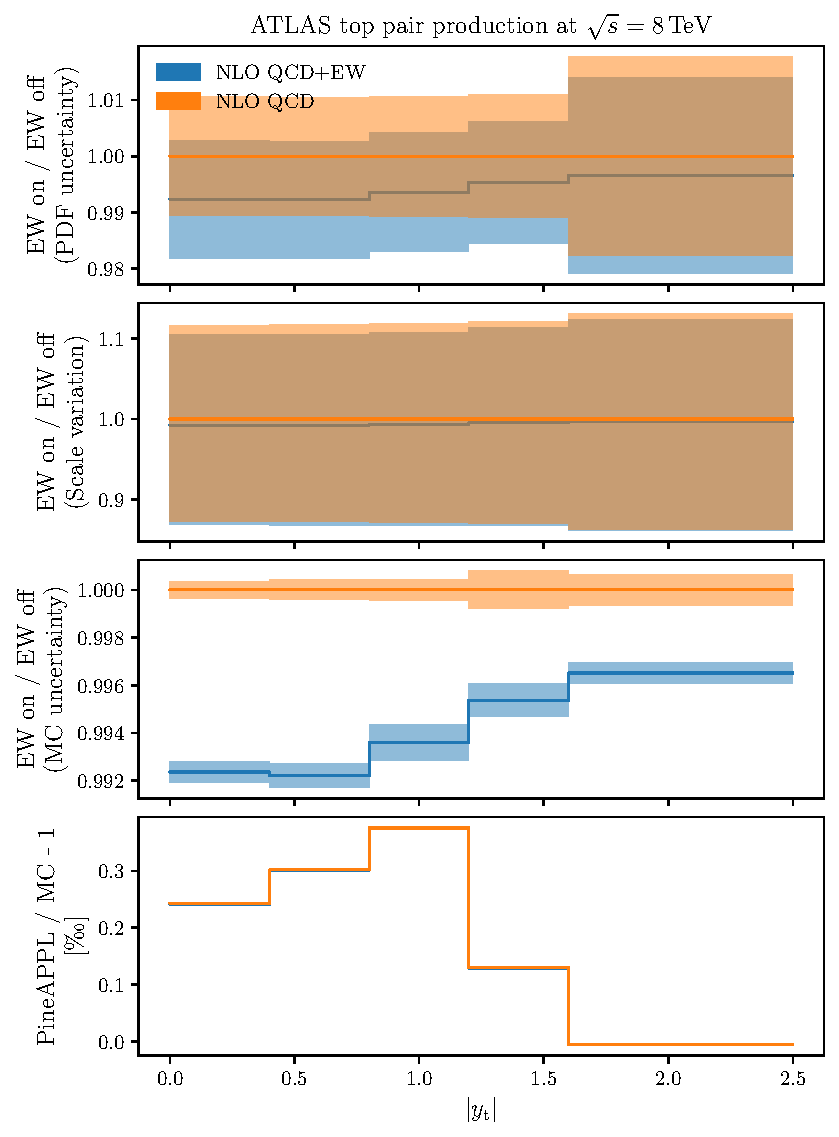
\includegraphics[width=0.46\textwidth]{figures/pineappl_ATLAS_TTB_DIFF_8TEV_LJ_TRAP}
    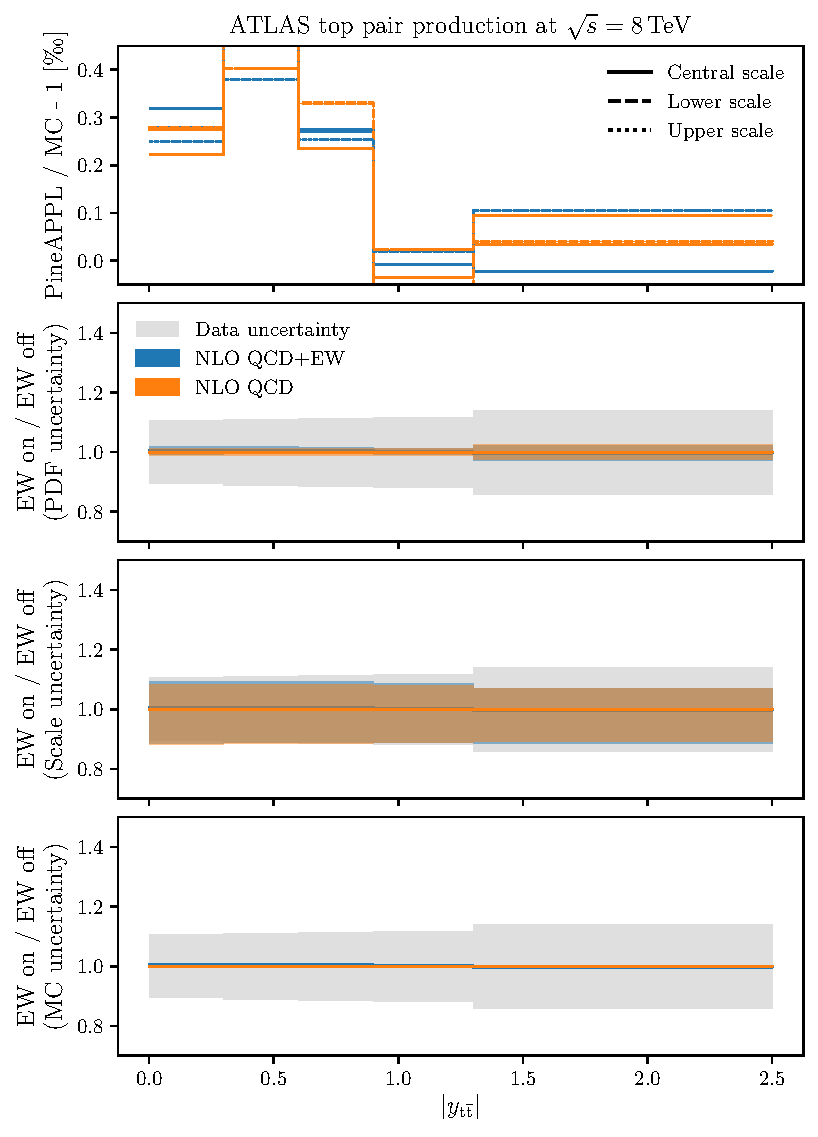
\includegraphics[width=0.46\textwidth]{figures/pineappl_ATLAS_TTB_DIFF_8TEV_LJ_TTRAP}\\
    \caption{Same as figure~\ref{fig:atlastop}, but for the distributions
      in the rapidity of the top quark, $y_{\mathrm{t}}$, and in the rapidity of
      the top-quark pair, $y_{\mathrm{t}\bar{\mathrm{t}}}$.}
    \label{fig:atlastop-rap}
\end{figure}
%-------------------------------------------------------------------------------

From figure~\ref{fig:atlaszhighmass49fb-lowstat}, we observe that the validation
of the \textsc{PineAPPL} result remains successful: its difference with respect
to the MC result is at most \SI{3}{\permille}, as usual irrespective of the
accuracy of the theory and of the choice of scale. As expected, however, the
result is largely unreliable to make any conclusion about the size of the EW
corrections: large fluctuations are seen in the predictions, and the MC
uncertainty dominates over the PDF and scale uncertainties.

Figure~\ref{fig:cmsdy2d11_bins12} demonstrates that the two bins at the
lowest invariant mass of the Drell--Yan lepton-pair measured by the CMS
experiment display very similar features as the bin at immediately larger
values of invariant mass, see figure~\ref{fig:cmsdy2d11_bins3456}: the EW
correction enhances the cross section by \SIrange{2}{3}{\percent} across all the
rapidity range; the amount of this shift is slightly larger than the PDF
uncertainty, but is largely overshot by the scale uncertainty; the MC
uncertainty remains comparatively negligible.

Finally, figure~\ref{fig:atlastop-rap} allows us to further validate the
\textsc{PineAPPL} result against the MC result for the top-quark
rapidity distributions, and to explicitly check that the size of the EW
corrections in this case is negligible with respect to the companion
top-quark transverse momentum and top-quark pair invariant mass distributions,
see figure~\ref{fig:atlastop}, consistently with what was already observed in
ref.~\cite{Czakon:2017wor}.
